\documentclass[../main/main.tex]{subfiles}
\graphicspath{{./figures/}}

\makeatletter
\renewcommand{\@chapapp}{Travaux pratiques -- TP}
\makeatother

\toggletrue{student}
\HideSolutionstrue

\begin{document}
\setcounter{chapter}{4}

\chapter{Oscilloscope et trac\'e de caract\'eristiques}

\ifstudent{
	\begin{prgm}
		\begin{tcb}*(ror)"know"{Savoirs}
			\begin{itemize}[label=$\diamond$, leftmargin=10pt]
				\item Préciser la perturbation induite par l'appareil de mesure sur le
				      montage et ses limites (bande passante, résistance d'entrée)~;
				\item Définir la nature de la mesure effectuée (valeur efficace, valeur
				      moyenne, amplitude, valeur crête à crête, etc.)~;
			\end{itemize}
		\end{tcb}
		\begin{tcb}*(ror)"how"{Savoir-faire}
			\begin{itemize}[label=$\diamond$, leftmargin=10pt]
				\item Mesurer une tension au voltmètre ou à l'oscilloscope~;
				\item Gérer, dans un circuit électronique, les contraintes liées à la
				      liaison entre les masses.
				\item Obtenir un signal de valeur moyenne, de forme, d’amplitude et de
				      fréquence données.
				\item Mettre en œuvre une méthode de mesure de fréquence ou de période.
			\end{itemize}
		\end{tcb}
	\end{prgm}
	\vspace{-10pt}
	\section{Objectifs}
	\begin{itemize}
		\item Se familiariser avec le GBF et l'oscilloscope numérique.
		\item Réaliser des montages simples d'électricité.
		      % \item Mesurer la résistance d'entrée $R_{e}$ d'un oscilloscope et la
		      %       résistance de sortie $R_{s}$ d'un GBF.
		\item Tracer une caractéristique de dipôle en utilisant un transformateur
		      d'isolement.
	\end{itemize}
}

\begin{tcb}[cnt](impo){}
	Vous prendrez soin de refaire tous les schémas des circuits mis en place ou
	étudiés.
\end{tcb}

\section{S'approprier}
\subsection{Résistances d'entrée et de sortie}

% Nous avons vu en TD la méthode dite de la «~demi-tension~» qui permet de
% mesurer la résistance d'entrée et de sortie d'un appareil (cf.\ exercice I TD
% 2, fait \textit{via} la puissance)

\subsubsection{Résistance de sortie du générateur basse fréquence (GBF)}

\begin{tcb}[sidebyside, righthand ratio=.35](defi){Résistance d'entrée}
	Le GBF est un générateur réel pouvant être modélisé comme une association
	série d'un générateur idéal de tension de force électromotrice $e$ associé à
	une résistance de sortie $r_{s}$ (modèle de \textsc{Thévenin}). Comme vu en
	cours, on branche le GBF sur une résistance variable $R'$ puis on mesure la
	tension $U_1$ aux bornes de $R'$.
	\tcblower
	\begin{center}
		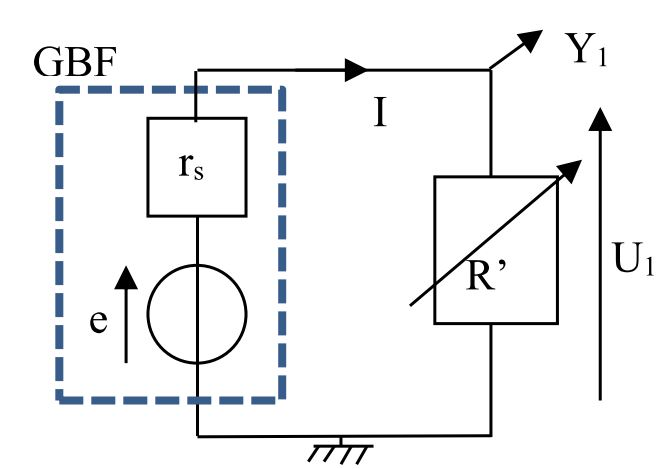
\includegraphics[width=\linewidth]{res_entree}
		\captionof{figure}{}
	\end{center}
\end{tcb}

\begin{enumerate}[label=\clenumi]
	\item Montrer que lorsque $U_1 = e/2$, alors $R' = r_{s}$.
	\item En déduire une méthode simple de mesure expérimentale de $r_{s}$.
\end{enumerate}

\begin{tcb}(expe){Aide}
	Afin de mesurer $U_1$, l'oscilloscope se branche entre la masse (reliée à la
	borne noire de l'oscilloscope) et le nœud $Y_1$ (relié à la borne rouge de
	l'oscilloscope). Notez que dans un circuit, \textbf{la masse est un nœud
		commun à tous les appareils branchés}.
	\smallbreak
	Par conséquent, la borne noire du GBF ainsi que les deux bornes noires de
	l'oscilloscope doivent être impérativement reliées entre elles. Si ce n'est
	pas le cas, votre montage ne fonctionnera pas.
\end{tcb}

\subsubsection{Résistance d'entrée de l'oscilloscope}

\begin{tcb}[sidebyside, righthand ratio=.35](defi){Résistance de sortie}
	L'entrée d'un oscilloscope est assimilable à une résistance d'entrée $R_{e}$
	en dérivation avec une capacité $C_{e}$. À \textbf{basse fréquence}, le
	condensateur est assimilable à un \textbf{interrupteur ouvert}, si bien que
	l'on peut dans un tel régime négligé sa présence.
	\tcblower
	\begin{center}
		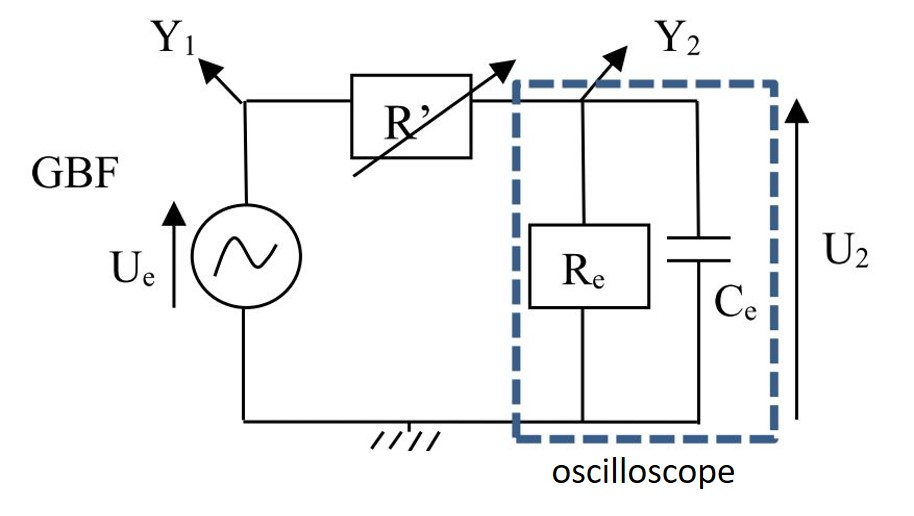
\includegraphics[width=\linewidth]{res_sortie}
		\captionof{figure}{}
	\end{center}
\end{tcb}

\begin{enumerate}[label=\clenumi, start=3]
	\item Montrer alors, en vous aidant du schéma, que la tension $U_2$, mesurée
	      par l'oscilloscope (modélisée par une résistance et une capacité en
	      parallèle), est égale à $U_{e}/2$ lorsque $R' = R_{e}$.
	\item En déduire une méthode simple de mesure expérimentale de $R_{e}$.
\end{enumerate}

\begin{tcb}(rema)<lfnt>{}
	Remarquez que, contrairement à ce qui est fait dans le cours, la résistance de
	sortie du GBF n'apparaît pas. Elle est en réalité très faible devant les
	autres résistances $R_{e}$ et $R'$ et sera donc négligée.
\end{tcb}

\subsection{Mesures avec un oscilloscope}

À partir du menu mesure, l'oscilloscope est capable de réaliser des mesures
automatiques des principales caractéristiques des signaux électriques. Vous
pourrez en particulier afficher~:

\begin{itemize}
	\item la période et la fréquence du signal~;
	\item la tension crête-crête $U_{\rm pp}$ du signal (valeur mesurée entre le
	      maximum et le minimum du signal)~;
	\item la tension efficace $U_{\rm eff}$ définie par
	      \encadre{$S_{\rm eff} = \sqrt{ \left\langle s^2(t) \right\rangle}
			      = \sqrt{\frac{1}{T}\int_{t_0}^{t_0+T} s^2(t) \dt}$}
\end{itemize}
\vspace{-10pt}
\begin{tcb}[sidebyside](defi){Amplitude et tensions}
	L'amplitude $A$ d'un signal (qui intervient dans l'expression d'un signal
	sinusoïdal selon $s(t) = A \cos(\omega t + \varphi)$) est liée à $U_{\rm
				pp}$ selon
	\[
		\boxed{A = U_{\rm pp}/2}
	\]
	\tcblower
	Par ailleurs, pour un signal sinusoïdal, \textbf{et uniquement pour un
		signal sinusoïdal} la tension efficace s'écrit~:
	\[
		\boxed{U_{\rm eff} = U_{\rm pp}/\sqrt{2} = \sqrt{2} A}
	\]
\end{tcb}

\begin{tcb}*[cnt, bld](prop)"bomb"{Attention}
	Pour toute mesure, vérifier que la source du menu mesure correspond bien à
	la courbe sur laquelle vous faites des mesures.
\end{tcb}

\subsection{Utilisation des oscilloscopes}
\subsubsection{Imprimer une courbe avec un oscilloscope \texttt{Rigol}}

\begin{enumerate}
	\item Allumer l'ordinateur et se connecter au réseau.
	\item Puis, programme, discipline, physique-chimie, physique, oscillo
	      \texttt{rigol}.
	\item \texttt{Tools}, \texttt{connect to oscillo}, puis \texttt{refresh}.
	\item Passer en noir et blanc (\texttt{B \& W}) et enfin \texttt{print}.
\end{enumerate}

\subsubsection{Imprimer une courbe avec un oscilloscope \texttt{Tektronix}}

\begin{enumerate}
	\item Ouvrir \texttt{Open Choice Desktop}. Sélectionner \texttt{instrument
		      USB} puis \texttt{Afficher écran}.
	\item Copier vers le presse-papier. Ouvrir \texttt{paint} et coller.
	\item Puis cliquer droit, inverser les couleurs.
	\item Sélection rectangulaire, pour ne garder que les oscillogrammes et les
	      réglages de l'oscilloscope.
	\item Copier~; Basculer dans \texttt{libre-office} ou \texttt{word} et
	      Coller~;
	\item Faire une belle mise en page et mettre des titres et commentaires
	      éventuels. Puis imprimer.
\end{enumerate}

\subsubsection{Incertitudes de lecture}
\begin{tcb}(rapp){Incertitudes composées à 2 variables~: somme ou différence}
	\[
		\boxed{
			y = x_1 \pm x_2
			\qquad \Ra \qquad
			u(y) = \sqrt{(u(x_1))^{2} + (u(x_2))^{2}}}
	\]
\end{tcb}

\section{Réaliser}
\subsection{Visualisation et mesures de tensions et période du signal}
% \subsubsection{}
\begin{tcb}(expe){Mesures de tension et période}
	\begin{enumerate}
		\item Brancher le GBF sur la voie 1 de l'oscilloscope~;
		\item Choisir une fréquence d'environ \SI{1000}{Hz} et une tension
		      sinusoïdale crête-crête de \SI{2}{V} (bouton DC offset enfoncé)~;
		\item Affichez la mesure de la tension \textit{via} l'oscilloscope en
		      sélectionnant $V_{pp}$ de la voie 1 (CH$_1$) dans le menu
		      \texttt{mesure}~;
		\item Régler le \textit{level} du GBF, tel que $V_{pp} = \SI{2}{V}$ pour
		      CH$_1$~;
		\item Visualiser le signal en réglant les vis d'échelles X et Y~;
		\item Mesurer la valeur maximale de tension ainsi que la période de la
		      tension en utilisant les règles de lectures et en règlant les
		      sensibilités de l'oscilloscope.
	\end{enumerate}
\end{tcb}
\begin{enumerate}[label=\sqenumi]
	\item Écrire les résultats en \si{mV} et \si{\micro s}. Vous ferez attention à
	      évaluer les incertitudes.
	      % \begin{tcb}(rapp)<lfnt>{}
	      %    Pour rappel, l'incertitude d'une différence ($t_2 - t_1$ par exemple)
	      %    se calcule par composition.
	      % \end{tcb}

	\item En déduire la tension efficace ainsi que la fréquence $f$ du signal.
	\item Dans le mesure \texttt{mesure}, lire directement les valeurs des
	      tensions $U_{\max}$, $U_{\rm eff}$ (notée $V_{\rm rms}$) et de la
	      période sur CH$_1$.
	\item Dans le menu \texttt{Trigger}, changer la source pour CH$_2$~: que
	      constatez-vous~?
	\item Revenez à la source 1, modifier le niveau de déclenchement. Quel est le
	      rôle de ce bouton~?
\end{enumerate}

\subsection{Tracé d'une caractéristique de résistor à l'oscilloscope}

\begin{tcb}[sidebyside, righthand ratio=.5](defi){Transformateur d'isolement}
	Dans le montage ci-contre, ce qui relie les deux circuits est un
	\textbf{transformateur d'isolement}. Il permet de reproduire à l'identique une
	tension sans utiliser de câble, comme présenté sur le schéma ci-contre.
	\smallbreak
	On se sert de ce dispositif pour imposer une nouvelle maille au circuit,
	permettant des mesures impossibles sinon.
	\tcblower
	\begin{center}
		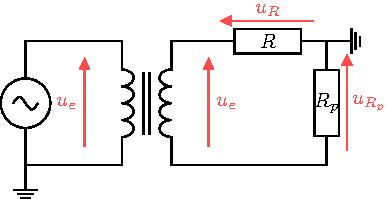
\includegraphics[width=\linewidth]{carac_r_oscillo}
		\captionof{figure}{}
		\label{fig:transfo}
	\end{center}
\end{tcb}
\begin{enumerate}[label=\clenumi, start=5]
	\item Retracer le circuit ci-contre, en enlevant le transformateur. La masse
	      étant imposée par le générateur, proposer des branchements et
	      manipulations pour observer $u_{R_p}$ sur la voie 1 et $u_R$ sur la
	      voie 2.
	\item Faire de même avec le circuit de la Figure~5.3. Conclure.
\end{enumerate}

\begin{tcb}(expe){Tracé d'une caractéristique}
	\begin{enumerate}
		\item Réaliser le montage précédent en utilisant le GBF, avec $f =
			      \SI{1}{kHz}$, \texttt{level} $\approx \SIrange{2}{3}{V}$, sans
		      offset, $R_P = \SI{100}{\omh}$ et $R$ \textit{inconnue}.
		\item Observer les 2 tensions à l'oscilloscope en centrant les deux voies.
	\end{enumerate}
\end{tcb}
\begin{enumerate}[label=\sqenumi, start=6]
	\item Visualise-t-on $u_{R_p}$ sans problème~? Que faut-il faire~?
	\item Imprimer les deux courbes en prenant \textbf{le même gain vertical}, et
	      \textbf{en déduire $R_{\rm inconnue}$}.
\end{enumerate}
\begin{tcb}(expe)<lfnt>{}
	\begin{enumerate}
		\item Dans le menu \texttt{horizontal}, passer en mode \texttt{XY}. On
		      visualise alors \texttt{CH2} en fonction de \texttt{CH1}, soit $u_R$
		      en fonction de $u_{R_p}$.
	\end{enumerate}
\end{tcb}
\begin{enumerate}[label=\sqenumi, start=8]
	\item Que représente cette courbe~? La figer avec le bouton \texttt{STOP} et
	      l'imprimer.
	\item En déduire la valeur de $R_{\rm inconnue}$ avec une autre méthode que
	      précédemment.
	\item Conclure sur leur compatibilité grâce à un écart normalisé.
\end{enumerate}
\begin{tcb}(rema)<lfnt>{}
	Pour prendre l'opposé d'un signal, dans le menu de la voie presser
	\faIcon{arrow-down}, puis activer \texttt{Inversée}.
\end{tcb}

% \section{Réaliser~: Résistances d'entrée et de sortie}
% \subsection{Mesure de la résistance de sortie du GBF}
%
% \begin{enumerate}
% 	\item Réaliser le montage vu dans la partie \textit{S'approprier} pour une
% 	      fréquence d'environ $\SI{100}{Hz}$ et commencer avec $R'$ infinie, donc
% 	      débranchée.
% 	\item Mesurer alors $U_1$ grâce à l'oscilloscope, et régler le
% 	      \texttt{level} du GBF (bouton DC offset enfoncé) pour obtenir une
% 	      tension crête-crête de $\SI{2}{V}$. Cette tension correspond à la
% 	      tension à vide $e$ du générateur. En effet, à vide, c'est-à-dire pour
% 	      $R'$ infinie, le courant est nul et donc la tension relevée est
% 	      directement égale à $e$.
% 	\item Brancher la boîte de résistances variables $R'$ et l'ajuster pour
% 	      avoir $U_1 = e/2$.
% 	\item En déduire l'ordre de grandeur de la résistance de sortie $r_{s}$ du
% 	      GBF.
% 	\item Cette valeur est-elle cohérente avec les indications inscrites sur la
% 	      sortie du GBF~?
% \end{enumerate}
%
% \vspace{-0.6cm}
%
% \subsection{Mesure de la résistance d'entrée de l'oscilloscope (modèle)}
%
% \begin{enumerate}
% 	\item Prendre la notice de l'oscilloscope dont vous disposez, vérifier les
% 	      valeurs de $R_{e}$ et $C_{e}$ appelées \textit{input impedance} en
% 	      anglais.
% 	\item Mesurer d'abord la tension $U_{e}$ en connectant directement
% 	      l'oscilloscope au générateur (cela revient à prendre une résistance $R'$
% 	      nulle, assimilable à un fil donc).
% 	\item Réaliser ensuite le montage présenté dans la partie
% 	      \textit{S'approprier}.
% 	\item $U_{e}$ étant fixé ($\SI{2}{V}$ crête-crête), faire varier $R'$
% 	      jusqu'à ce que la tension aux bornes de l'oscilloscope ($U_2$) soit
% 	      égale à la moitié de la tension du générateur $U_{e}$. Vous pouvez
% 	      utiliser le menu mesure pour obtenir la valeur des deux tensions.
% 	\item En déduire l'ordre de grandeur de la résistance d'entrée $R_{e}$
% 	      expérimentale de l'oscilloscope.
% \end{enumerate}
%
\section{Valider} %~: Effets des résistances d'entrée et de sortie}
\subsection{Effet de la résistance de sortie du GBF}

Brancher l'oscilloscope aux bornes du GBF (toujours réglé à une fréquence de
$\SI{1}{kHz}$) et régler le \texttt{level} de celui-ci pour obtenir une tension
crête-crête de $\SI{2}{V}$. Comme précédemment, nous mesurons ici la tension à
vide $e$ du GBF.

\noindent
\begin{minipage}[t]{.65\linewidth}
	\begin{enumerate}[label=\sqenumi, start=10]
		\item Brancher aux bornes du GBF deux résistances identiques de
		      $R_1 = R_2 = \SI{47}{\Omega}$ en série. Faire un schéma, puis relever
		      à l'aide de l'oscilloscope la tension $U_2$ aux bornes de $R_2$.
		\item En appliquant le principe du pont diviseur de tension, que devrait
		      valoir $U_2$~? Est-ce la valeur que vous relevez~?
		\item Expliquez cet écart en considérant la résistance de sortie du GBF.
		\item Comment choisir $R_1$ et $R_2$ pour que l'on puisse négliger l'effet
		      de la résistance de sortie du GBF~? Reproduire le montage précédent en
		      utilisant désormais $R_1 = R_2 = \SI{10}{k\Omega}$. Montrer qu'alors
		      $U_1$ prend la valeur attendue.
		\item Pourrait-on brancher l’oscilloscope aux bornes de $R_1$~? Justifier.
	\end{enumerate}
\end{minipage}
\hfill
\begin{minipage}[t]{.35\linewidth}
	~
	\vspace{-20pt}
	\begin{center}
		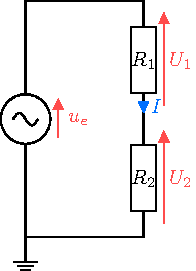
\includegraphics[width=.8\linewidth]{divis_tension}
		\captionof{figure}{}
	\end{center}
\end{minipage}

\subsection{Effet de la résistance d'entrée de l'oscilloscope}

\begin{enumerate}[label=\sqenumi, start=15]
	\item Brancher l'oscilloscope aux bornes du GBF (toujours réglé à une
	      fréquence de $\SI{1}{kHz}$) et régler le \texttt{level} de celui-ci
	      pour obtenir une tension crête-crête de $\SI{4}{V}$. Comme précédemment,
	      nous mesurons ici la tension à vide $e$ du GBF.
	\item Brancher aux bornes du GBF deux résistances identiques de $R_1 = R_2 =
		      \SI{1}{M\Omega}$ en série puis relever à l'aide de l'oscilloscope la
	      tension $U_1$ aux bornes de l'une d'elle.
	\item La tension $U_1$ obtenue est-elle conforme à vos attentes~? Expliquez
	      cet écart en tenant compte de la résistance d'entrée de l'oscilloscope.
	\item Comment choisir $R_1$ et $R_2$ pour que l'on puisse négliger l'effet
	      de la résistance d'entrée de l'oscilloscope~? Reproduire le montage
	      précédent en utilisant désormais $R_1 = R_2 = \SI{10}{k\Omega}$. Montrer
	      qu'alors $U_1$ prend la valeur attendue.
\end{enumerate}

\section{Conclure}

\begin{enumerate}[label=\sqenumi, start=19]
	\item Résumer les recommandations pratiques que vous avez pu déduire de ce TP
	      afin de réaliser des mesures correctes en électricité.
\end{enumerate}


\end{document}
